\documentclass{article}

\usepackage{neurips_2026}

\usepackage[utf8]{inputenc}
\usepackage[T1]{fontenc}
\usepackage{hyperref}
\usepackage{url}
\usepackage{booktabs}
\usepackage{amsfonts}
\usepackage{amsmath}
\usepackage{nicefrac}
\usepackage{microtype}
\usepackage{xcolor}
\usepackage{graphicx}
\usepackage{multirow}

% ---------------------------------------------------------------
\title{Deep Reinforcement Learning for Compiler Optimization\\
       Pass Ordering in LLVM}

% ================================================================
% SUBMISSION VERSION (double-blind)
% ================================================================
\author{Anonymous Author(s)}

% ================================================================
% CAMERA-READY VERSION: comment out the block above and uncomment
% this block after acceptance.
% ================================================================
% \author{%
%   Wei-Hsuan Tai$^1$ \And
%   Ting-Xuan Ma$^2$ \And
%   Yu-Siang Deng$^2$ \And
%   Shang-Che Li$^2$ \And
%   Wei-Chung Lu$^3$ \\[4pt]
%   $^1$Department of Biomedical Engineering,
%   National Taiwan University \\
%   $^2$Department of Computer Science and Information Engineering,
%   National Taiwan University \\
%   $^3$Graduate Institute of Networking and Multimedia,
%   National Taiwan University \\
%   Taipei, Taiwan \\
%   \texttt{\{b12508026, b12902003, b12902004, b12902033, r14944011\}@ntu.edu.tw}
% }

\begin{document}

\maketitle

% ---------------------------------------------------------------
\begin{abstract}
The phase ordering problem---determining the optimal sequence of compiler
optimization passes---is NP-hard and has resisted efficient exact solutions for
decades.  We investigate how far traditional deep reinforcement learning (DRL)
can be pushed on this problem without relying on large language models or
hand-crafted heuristics, using the CompilerGym~\cite{CompilerGym} LLVM
environment as our testbed.

Our work makes three contributions.
First, through a systematic ablation of six state representations, we identify
\emph{pass\_sequence}---encoding the ordered history of the $k$ most recent
optimization passes as concatenated one-hot vectors---as the strongest representation in our evaluated design space, outperforming IR-feature-based (Autophase) and count-based
alternatives by a large margin.
Second, we develop a scalable training infrastructure with truncation-aware
Generalized Advantage Estimation~\cite{schulman2015high}, 8-worker parallel
rollout collection (7.6$\times$ speedup), and per-suite reward normalization
for stable multi-suite joint training.
Third, an inference-time ensemble of seven independently trained policies with
best-of-8 stochastic rollouts achieves mean reward 1.050 on \texttt{cbench-v1}
and beats \texttt{-Oz} on 20 out of 23 programs---doubling the count compared
to our recurrent PPO baseline (10/23).  A single-model best-of-16 policy
reaches mean reward 1.060 and beats \texttt{-Oz} on 21 out of 23 programs
using only 16 rollouts, outperforming a random best-of-56 baseline (0.992
mean reward, 5/23 programs) under a controlled compute budget.  Cross-suite
evaluation across six additional benchmark suites demonstrates zero-shot
generalization.
\end{abstract}


% ---------------------------------------------------------------
\section{Introduction}

The phase ordering problem is a fundamental challenge in compiler optimization:
it asks for the optimal ordering of compilation passes such that the resulting
low-level code achieves the best performance or the smallest code size.
Different pass orderings can produce substantially different machine code,
making the choice of optimization schedule particularly consequential in
performance-critical settings.
Despite decades of research, the problem remains NP-hard in the general case,
and no efficient algorithm is known to find globally optimal pass sequences.

Classical solutions rely on fixed schedules (\texttt{-O2}, \texttt{-O3},
\texttt{-Oz}) that represent manually tuned compromises over a broad class of
programs.  While effective in practice, these schedules cannot adapt to the
structure of individual programs, leaving program-specific optimization
opportunities unexploited.  Iterative compilation methods search the pass-order
space exhaustively but scale poorly.

The recent rise of reinforcement learning (RL) offers a natural fit: an agent
can interact with the compiler step by step, observe the evolving intermediate
representation, and learn a policy that selects passes sequentially.
To facilitate such approaches, CompilerGym~\cite{CompilerGym} provides a
standardized gym-compatible interface to LLVM optimization with reproducible
benchmarks and objective reward signals.

Despite this promise, recent work has moved toward large language model
(LLM)-based approaches~\cite{pan2026compiler}, which require orders of
magnitude more compute and sacrifice the sample efficiency of actor-critic
methods.  This paper instead investigates how far \emph{traditional} DRL can
be pushed, focusing on two questions: (1)~\emph{what is the best way to
represent the compiler state for a DRL agent?} and (2)~\emph{how can
inference-time diversity be exploited to further improve performance without
additional training cost?}

We make the following contributions:
\begin{itemize}
  \item \textbf{State representation study.}  A controlled ablation of six
        representations shows that \texttt{pass\_sequence} ($k{=}10$)---encoding
        the ordered history of recent passes---is the dominant design choice
        (avg reward $0.510\to0.937$ over normalized Autophase).
  \item \textbf{Scalable training infrastructure.}  Truncation-aware GAE,
        8-worker parallel rollouts, and per-suite Welford normalization enable
        stable multi-suite training across suites with up to $42\times$ reward
        variance ratio.
  \item \textbf{Inference-time ensemble.}  Seven independently trained policies
        with bo8 rollouts achieve avg 1.050 on \texttt{cbench-v1} (20/23
        $\geq$\texttt{-Oz}), generalizing zero-shot to six additional suites.
  \item \textbf{Compute-budget comparison.}  MLP-Seq-Full (bo16) (16 rollouts,
        avg 1.060, 21/23~$\geq$\texttt{-Oz}) outperforms random best-of-56
        (56 rollouts, avg 0.992, 5/23) on all 23 benchmarks.
\end{itemize}


% ---------------------------------------------------------------
\section{Related Work}

\subsection{Compiler Optimization as a Sequential Decision Problem}

Early iterative-compilation systems such as MILEPOST~\cite{fursin2011milepost}
treated pass ordering as a supervised or genetic-search problem with offline
models that cannot adapt at inference time.
CompilerGym~\cite{CompilerGym} formalizes the problem as a Markov Decision
Process, providing a gym-compatible interface with objective reward signals.
Our work builds directly on this framework.

\subsection{Reinforcement Learning for Compiler Optimization}

Huang et al.~\cite{8735549} introduced Autophase, a 56-dimensional IR feature
vector, and showed that a simple RL agent trained on it can surpass fixed
optimization levels on individual programs.
Cummins et al.~\cite{cummins2021programl} proposed graph-based IR
representations (ProGraML) for learning program structure at higher training
cost.
Compiler-R1~\cite{pan2026compiler} applies LLMs with reinforcement fine-tuning,
achieving strong results at orders-of-magnitude higher compute.
Our work establishes a strong traditional-DRL baseline and a systematic
understanding of what representations and inference strategies matter most.

\subsection{PPO, ICM, and Ensemble Methods}
PPO~\cite{schulman2017proximal} is applied to combinatorial action spaces
including chip placement~\cite{mirhoseini2021graph}; we adopt MLP (ablation)
and recurrent GRU (ensemble) variants.
ICM~\cite{pathak2017curiosity} adds a prediction-error exploration bonus;
in our setup the signal decays to negligible magnitude by mid-training.
Ensemble methods~\cite{lakshminarayanan2017simple, osband2016deep} exploit
policy diversity; each run converges to a different attractor, and the
per-program max recovers the best-fitting policy at inference time.


% ---------------------------------------------------------------
\section{Methodology}

Our investigation proceeds in two phases.
\textbf{Phase~1} (Section~4.2--4.5) conducts controlled ablations using
the full 124-pass action space and a feed-forward MLP to identify the
optimal state representation.
\textbf{Phase~2} (Section~4.6--4.7) scales up with a recurrent GRU policy,
curated 30-pass action set, parallel rollouts, and an inference-time ensemble.
The key insight from Phase~1---that sequential pass history is the most
informative signal---motivates the history-augmented state in Phase~2.

\subsection{MDP Formulation}

\paragraph{State.}
We evaluate two families of state representations (detailed in
Section~\ref{sec:ablation}).

\textit{Pass-sequence encoding} (\texttt{pass\_sequence}, $k$): the ordered
history of the $k$ most recent passes, encoded as a concatenation of $k$
one-hot vectors over the 124-pass action space, yielding $k \times 124$
dimensions.  Episodes shorter than $k$ steps are zero-padded at the front.
This is the best-performing representation identified by our ablation
($k{=}10$, 1240-dim).

\textit{Autophase with per-action usage counts}: the 56-dimensional Autophase
vector~\cite{8735549}, per-feature online normalized via a Welford estimator
$\hat{\phi}_i = (\phi_i - \mu_i)/(\sigma_i + \epsilon)$, concatenated with a
vector recording how many times each pass has been applied this episode.  This
representation is used in the recurrent ensemble model (Phase~2), where the GRU
hidden state additionally models pass-interaction history.

\paragraph{Action.}
Phase~1 uses the full 124-pass LLVM action space.  Phase~2 uses a curated
30-pass subset (PASSES\_V4) derived from the \texttt{-Oz} pass schedule,
which reduces the search space while retaining the most effective passes.

\paragraph{Reward.}
Both phases use the \texttt{IrInstructionCountOz} reward, which is
implemented as a \emph{per-step} incremental signal:
\begin{equation}
  r_t = \frac{\mathrm{IC}(P_{t-1}) - \mathrm{IC}(P_t)}
             {\max\!\bigl(\mathrm{IC}_{-O0}(P) - \mathrm{IC}_{-Oz}(P),\; 1\bigr)},
  \label{eq:reward}
\end{equation}
where $\mathrm{IC}(P_t)$ is the IR instruction count after applying pass
$a_t$, and the denominator normalizes by the improvement that
$\texttt{-Oz}$ achieves over $\texttt{-O0}$ (the unoptimized baseline).
The first step initializes $\mathrm{IC}(P_0) = \mathrm{IC}_{-O0}(P)$.

Because Eq.~(\ref{eq:reward}) is a telescoping sum, the cumulative episode
reward simplifies to:
\begin{equation}
  R = \sum_{t=1}^{T} r_t
    = \frac{\mathrm{IC}_{-O0}(P) - \mathrm{IC}(P_T)}
           {\mathrm{IC}_{-O0}(P) - \mathrm{IC}_{-Oz}(P)},
\end{equation}
where $P_T$ is the final program after the agent's pass sequence.
$R = 1.0$ means the agent matches $\texttt{-Oz}$; $R > 1.0$ means it
surpasses $\texttt{-Oz}$; $R < 0$ means the agent performs worse than
the unoptimized $\texttt{-O0}$ baseline.

\paragraph{POMDP structure.}
Compiler pass ordering is a POMDP: Autophase provides only a partial observation,
causing state aliasing---identical observations may require different actions
depending on transformation history.  \texttt{pass\_sequence} approximates the
belief state $b_t{=}P(s_t{\mid}o_1,a_1,\ldots,o_t)$ by supplying the last $k$
actions as an explicit history signal, explaining the gap between
autophase\_norm (avg 0.510) and pass\_sequence (avg 0.937).

\paragraph{Episode length.}
$T = 45$ steps maximum (TimeLimit wrapper).  Extending to $T = 90$ degraded
performance, confirming that the binding constraint is the action set, not
the time budget.

\subsection{Phase 1: Feed-Forward MLP Policy}

For ablation studies, we use a two-layer MLP (256$\times$256, ReLU) as the
actor-critic backbone.  The MLP takes the state representation directly as
input and outputs a logit vector over the action space and a scalar value
estimate.  This non-recurrent architecture is deliberately simple to isolate
the effect of the state representation.

\subsection{Phase 2: Recurrent GRU Policy with ICM}
\label{sec:phase2}

For ensemble training, we use a recurrent actor-critic with a GRU backbone.
The state $s'_t$ is encoded by an MLP with LayerNorm and GELU activations:
$\phi_t = f^{\mathrm{enc}}_{\theta}(s'_t)$.
The GRU conditions on both the latent state and the previous action,
$h_t = \mathrm{GRU}([\phi_t \| a_{t-1}^{\mathrm{onehot}}],\, h_{t-1})$,
enabling the policy to reason about transformation history in this POMDP setting.
The shared $h_t$ feeds actor and critic heads:
\begin{equation}
  \pi_{\theta}(a_t \mid h_t) = \mathrm{softmax}(f^{\pi}_{\theta}(h_t)),
  \qquad
  V_{\theta}(s_t) = f^{v}_{\theta}(h_t).
\end{equation}

\paragraph{Intrinsic Curiosity Module (ICM).}
To encourage early-training exploration, we augment the extrinsic reward with
an ICM~\cite{pathak2017curiosity} bonus.  A forward model predicts
$\hat{\phi}_{t+1} = g^{\mathrm{fwd}}_\psi(\phi_t, a_t)$ and produces
intrinsic reward $r_t^{\mathrm{int}} = \tfrac{1}{2}\|\hat{\phi}_{t+1} - \phi_{t+1}\|^2$.
An inverse model $g^{\mathrm{inv}}_\psi(\phi_t, \phi_{t+1})$ is trained via
cross-entropy loss to preserve action-predictive information in $\phi_t$.
The total reward is $r'_t = r_t^{\mathrm{ext}} + \beta r_t^{\mathrm{int}}$;
empirically, the ICM signal decays to negligible magnitude by mid-training.

\subsection{PPO Training and Truncation-Aware GAE}

We train the agent using PPO~\cite{schulman2017proximal} with the clipped
surrogate objective:
\begin{equation}
  \mathcal{L}_{\mathrm{PPO}}
  = \mathbb{E}_t\!\left[
    \min\!\left(
      \rho_t A_t,\;
      \mathrm{clip}(\rho_t,\, 1{-}\epsilon,\, 1{+}\epsilon)\, A_t
    \right)
  \right],
\end{equation}
where $\rho_t = \pi_\theta(a_t|s_t)/\pi_{\theta_{\mathrm{old}}}(a_t|s_t)$
is the probability ratio and $A_t$ is the GAE advantage estimate.

Standard GAE~\cite{schulman2015high} sets the bootstrap value to zero at
terminal states.  When an episode ends by time-limit truncation rather than
a true terminal transition, the correct target is $V(s_T)$, not zero.  We
maintain a truncation buffer that distinguishes truncated from truly terminal
transitions, bootstrapping $V(s_T)$ at truncation boundaries.  This
eliminates a systematic underestimation of long-horizon credit.

\subsection{Parallel Rollout Collection}

We use $W{=}8$ parallel workers in a synchronous actor-learner
architecture.  Each worker maintains an independent CompilerGym gRPC service;
the main process broadcasts weights and normalization statistics before each
collection phase.  The first transition per worker is flagged as a new episode
boundary to reset the GRU hidden state.  This reduces training from
$\approx$3 hours to 47 minutes per 300k steps (7.6$\times$ speedup).

\subsection{Inference-Time Ensemble}

Given $N$ checkpoints $\{\pi_1,\ldots,\pi_N\}$ and rollout budget $k$ per
model, the ensemble selects for each program $p$:
\begin{equation}
  \hat{R}(p) = \max_{i \in [N],\; j \in [k]}
               R\!\left(\tau_{i,j}(p)\right).
\end{equation}
We set $k{=}8$ (bo8) and $N \in \{5,6,7\}$.  Each run---with distinct
learning rate, entropy coefficient, or state-feature configuration---converges
to a different attractor~\cite{lakshminarayanan2017simple, osband2016deep};
the per-program maximum recovers the best-fitting attractor at inference time
with no training cost.

\subsection{Per-Suite Reward Normalization}

Joint training causes per-step rewards to span $[-30,+5]$, leading to
value-loss divergence at step 80k.  We apply a per-suite Welford z-score:
$\tilde{r}_t^{(s)} = \mathrm{clip}((r_t^{(s)}{-}\mu^{(s)})/(\sigma^{(s)}{+}\epsilon),\,-5,\,+5)$.
This keeps value loss in $[0.2, 0.8]$ across 300k steps despite a
$42\times$ per-suite reward variance ratio (cbench $\sigma{=}0.11$,
opencv $\sigma{=}4.44$).


% ---------------------------------------------------------------
\section{Experiments}

\subsection{Setup}

\paragraph{Environment.}
We use CompilerGym~\cite{CompilerGym} \texttt{llvm-v0} with the
\texttt{IrInstructionCountOz} reward.
\texttt{cbench-v1} is a standard compiler benchmark suite comprising 23~C
programs spanning embedded workloads (cryptography, image processing, data
compression, string search, and networking).
All models are \textbf{trained exclusively on cbench-v1} and evaluated both
in-distribution (cbench-v1) and zero-shot on six held-out suites: mibench-v1,
blas-v0, npb-v0, chstone-v0, opencv-v0, and anghabench-v1, covering linear
algebra kernels, HPC benchmarks, and large open-source C codebases.

\paragraph{Algorithm.}
PPO~\cite{schulman2017proximal}: clip $\varepsilon{=}0.2$, $\gamma{=}0.99$,
GAE $\lambda{=}0.95$~\cite{schulman2015high}, $n\_\text{steps}{=}512$,
entropy\_coef$=0.01$, value\_coef$=0.5$, lr$=3\times10^{-4}$.

\paragraph{Hardware.}
Phase~1: NVIDIA RTX 5070 Ti (500 ep/benchmark).
Phase~2: Apple Mac mini M4 Pro, 24\,GB, 8 CPU workers, $\approx$47 min/300k steps.

\paragraph{Baselines.}
\textbf{Random} (greedy); \textbf{Random best-of-56} (budget-controlled);
\textbf{-O3} (deterministic, single-shot);
\textbf{PPO-Baseline}: recurrent PPO, 15-pass action set, raw Autophase, 200k steps.

% ----------
\subsection{State Representation Ablation}
\label{sec:ablation}

\begin{figure}[h]
  \centering
  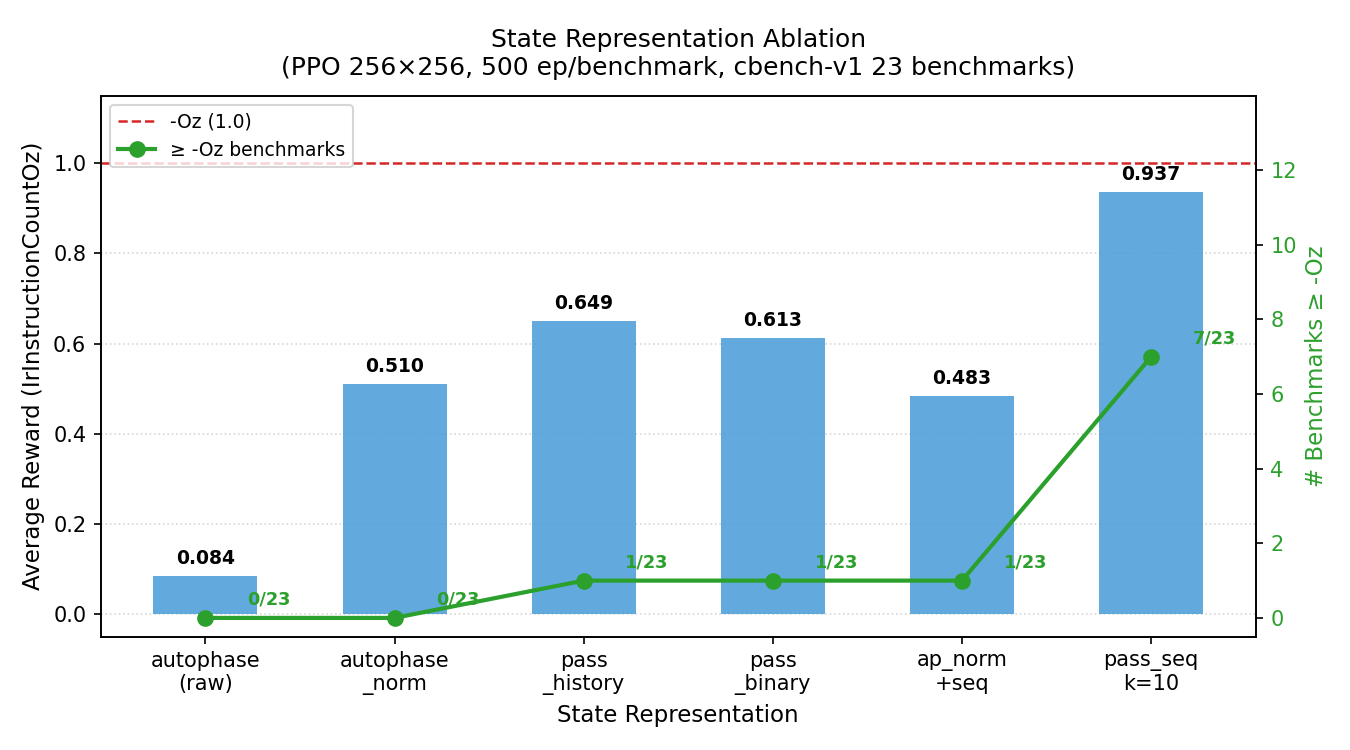
\includegraphics[width=0.85\linewidth]{figures/state_ablation.png}
  \caption{Average reward (left axis, blue bars) and number of programs
           beating \texttt{-Oz} (right axis, green line) for each state
           representation (23 \texttt{cbench-v1} benchmarks, greedy rollout).
           \texttt{pass\_sequence} ($k{=}10$) substantially outperforms all
           alternatives; the red dashed line marks the \texttt{-Oz} parity
           level ($R{=}1.0$).}
  \label{fig:state_ablation}
\end{figure}

\begin{table}[h]
  \caption{State representation ablation (256$\times$256 MLP, 500 episodes,
           greedy rollout, all 23 \texttt{cbench-v1} benchmarks).}
  \label{tab:state}
  \centering
  \begin{tabular}{lcrcc}
    \toprule
    Representation & Dim & Avg Reward & $\geq$Oz & $\geq$O3 \\
    \midrule
    autophase (raw)          & 56   & 0.084 & 0/23 & 2/23  \\
    autophase\_norm (log1p)  & 56   & 0.510 & 0/23 & 9/23  \\
    pass\_binary             & 124  & 0.613 & 1/23 & 14/23 \\
    pass\_history            & 124  & 0.649 & 1/23 & 11/23 \\
    autophase\_norm+sequence & 1296 & 0.484 & 1/23 & 8/23  \\
    \textbf{pass\_sequence ($k{=}10$)} & \textbf{1240} &
      \textbf{0.937} & \textbf{7/23} & \textbf{22/23} \\
    \bottomrule
  \end{tabular}
\end{table}

Table~\ref{tab:state} reveals a decisive hierarchy.
\textbf{autophase (raw)} collapses to near-zero: raw IR values reach 89,000+,
causing gradient overflow (avg 0.084 across 23 benchmarks).  \textbf{autophase\_norm} recovers learning but
lacks action-history context.  \textbf{pass\_binary} and
\textbf{pass\_history} encode which passes were applied but discard ordering
information.  \textbf{autophase\_norm+sequence} (1296-dim combined, avg 0.484) hurts
relative to sequence alone: the high-dimensional input exceeds the 500-episode
sample budget.  \textbf{pass\_sequence} ($k{=}10$, 1240-dim), encoding the
ordered history of the most recent $k$ passes as concatenated one-hot vectors,
outperforms all alternatives---7/23 programs beat \texttt{-Oz} and 22/23 beat
\texttt{-O3}.  The key insight is that \emph{pass order}, not just IR state or
pass membership, is the critical information for the agent.

% ----------
\subsection{Sequence Window, Architecture, and Hyperparameter Ablations}

\begin{table}[h]
  \caption{Ablations on window $k$, network size, and PPO hyperparameters
           (all 23 \texttt{cbench-v1} benchmarks).
           Base config: pass\_sequence, 256$\times$256 MLP, $k{=}10$,
           n\_steps$=512$, ent$=0.01$.}
  \label{tab:ablations}
  \centering
  \begin{tabular}{llrcc}
    \toprule
    Factor & Setting & Avg Reward & $\geq$Oz & $\geq$O3 \\
    \midrule
    \multirow{4}{*}{Window $k$}
      & $k=3$  (372-dim)  & 0.704 & 1/23 & 18/23 \\
      & $k=5$  (620-dim)  & 0.741 & 1/23 & 20/23 \\
      & \textbf{$k=10$ (1240-dim)} & \textbf{0.937} & \textbf{7/23} & \textbf{22/23} \\
      & $k=20$ (2480-dim) & 0.726 & 2/23 & 17/23 \\
    \midrule
    \multirow{2}{*}{Network}
      & \textbf{256$\times$256} ($\sim$1.1M)   & \textbf{0.937} & \textbf{7/23} & \textbf{22/23} \\
      & 512$\times$512 ($\sim$4.2M)   & 0.731 & 3/23 & 18/23 \\
    \midrule
    \multirow{3}{*}{PPO params}
      & \textbf{n\_steps=512, ent=0.01} & \textbf{0.937} & \textbf{7/23} & \textbf{22/23} \\
      & n\_steps=2048             & 0.722 & 1/23 & 20/23 \\
      & entropy\_coef=0.05        & 0.778 & 2/23 & 21/23 \\
    \bottomrule
  \end{tabular}
\end{table}

$k{=}10$ is optimal: shorter windows lack ordering context; $k{=}20$ (2480-dim)
exceeds the 500-episode sample budget.  Larger networks hurt for the same
reason---256$\times$256 ($\sim$1.1M params) balances capacity and efficiency.
Increasing n\_steps to 2048 reduces PPO updates from $\sim$43 to $\sim$11 per
run, severely limiting learning.  High entropy (0.05) over-explores and
prevents exploitation.

\paragraph{Reward alignment.}
Training with \texttt{IrInstructionCountO3} instead of \texttt{IrInstructionCountOz}
yields avg 0.715 on the \texttt{-Oz} evaluation metric (vs.\ 0.937 for Oz-trained),
confirming that training and evaluation objectives must match.

% ----------
\subsection{Cross-Architecture Validation of pass\_sequence}
\label{sec:crossarch}

To verify that pass\_sequence is broadly beneficial and not an artifact of our
MLP architecture, we evaluate it in the GRU-based policy (Phase~2) by
comparing GRU-Base (GRU + 30-pass, no sequence feature) against GRU-Seq (GRU + 30-pass
+ pass\_sequence $k{=}10$) and GRU-Seq-Full (GRU + full 124-pass + pass\_sequence
$k{=}10$).

\begin{table}[h]
  \caption{Cross-architecture comparison on all 23 \texttt{cbench-v1}
           benchmarks (greedy unless noted).  GRU-Base/GRU-Seq/GRU-Seq-Full use the GRU + ICM
           Phase~2 architecture; ours uses the MLP Phase~1 architecture.}
  \label{tab:crossarch}
  \centering
  \begin{tabular}{llccc}
    \toprule
    Method & Action Set & State Dim & Avg & $\geq$Oz \\
    \midrule
    GRU-Base          & 30-pass       & 87   & 0.999 &  9/23 \\
    GRU-Seq   & 30-pass       & 387  & 1.038 & 12/23 \\
    GRU-Seq (bo16)                   & 30-pass       & 387  & 1.050 & 18/23 \\
    GRU-Seq-Full   & 124-pass      & 1421 & 0.956 &  2/23 \\
    \midrule
    MLP-Seq-Full & 124-pass      & 1240 & 0.937 &  7/23 \\
    \textbf{MLP-Seq-Full (bo16)}        & \textbf{124-pass} & \textbf{1240} &
      \textbf{1.060} & \textbf{21/23} \\
    \bottomrule
  \end{tabular}
\end{table}

Table~\ref{tab:crossarch} and Figure~\ref{fig:perbench} yield three insights.
(1)~\textbf{pass\_sequence generalizes across architectures}: GRU-Base$\to$GRU-Seq gains
$+3.9$pp greedy avg and $+3$~$\geq$Oz purely from adding the sequence feature,
confirming the ablation result is architecture-independent.
(2)~\textbf{Curated action set enables strong greedy}: both GRU-Seq-Full (GRU, 124-pass,
0.956) and ours (MLP, 124-pass, 0.937) underperform GRU-Seq (1.038);
the full 124-pass space contains useless passes that destabilize greedy selection.
(3)~\textbf{Stochastic inference gains depend on action-space size}:
GRU-Seq (bo16) gains only $+1.2$pp ($1.038\to1.050$, $+6$~$\geq$Oz) over
greedy because the curated set already finds strong sequences.
MLP-Seq-Full (bo16) gains $+12.3$pp ($0.937\to1.060$, $+14$~$\geq$Oz)
because the larger 124-pass space provides diversity to recover hard benchmarks.
MLP-Seq-Full (bo16, 21/23~$\geq$Oz) thus outperforms GRU-Seq (bo16, 18/23)
despite its weaker greedy baseline---the action-space breadth is the decisive factor.

% ----------
\subsection{Best-of-$N$ Inference and Compute-Budget Comparison}

\begin{table}[h]
  \caption{Full results on \texttt{cbench-v1} (23 benchmarks).
           Rollouts: inference-time compiler invocations per program.
           Random best-of-56 is the compute-budget-matched baseline for
           ens7 ($7{\times}8{=}56$).  Phase~1: MLP; Phase~2: GRU+ICM.}
  \label{tab:main}
  \centering
  \begin{tabular}{llcc}
    \toprule
    Method & Rollouts & Avg Reward & $\geq$Oz \\
    \midrule
    Random (greedy)                    &  1 & 0.681 &  0/23 \\
    Random best-of-56                  & 56 & 0.992 &  5/23 \\
    PPO-Baseline                  &  1 & 1.015 & 10/23 \\
    \midrule
    \multicolumn{4}{l}{\textit{Phase~1: MLP-Seq-Full}} \\
    \quad greedy                       &  1 & 0.937 &  7/23 \\
    \quad \textbf{bo16}                & \textbf{16} &
      \textbf{1.060} & \textbf{21/23} \\
    \midrule
    \multicolumn{4}{l}{\textit{Phase~2: GRU-Base / GRU-Seq}} \\
    \quad GRU-Seq (greedy)   &  1 & 1.038 & 12/23 \\
    \quad GRU-Seq (bo16)                      & 16 & 1.050 & 18/23 \\
    \quad Ensemble ens5 ($N{=}5$, bo8) & 40 & 1.050 & 20/23 \\
    \quad Ensemble ens7 ($N{=}7$, bo8) & 56 & 1.049 & 19/23 \\
    \bottomrule
  \end{tabular}
\end{table}

\begin{figure}[h]
  \centering
  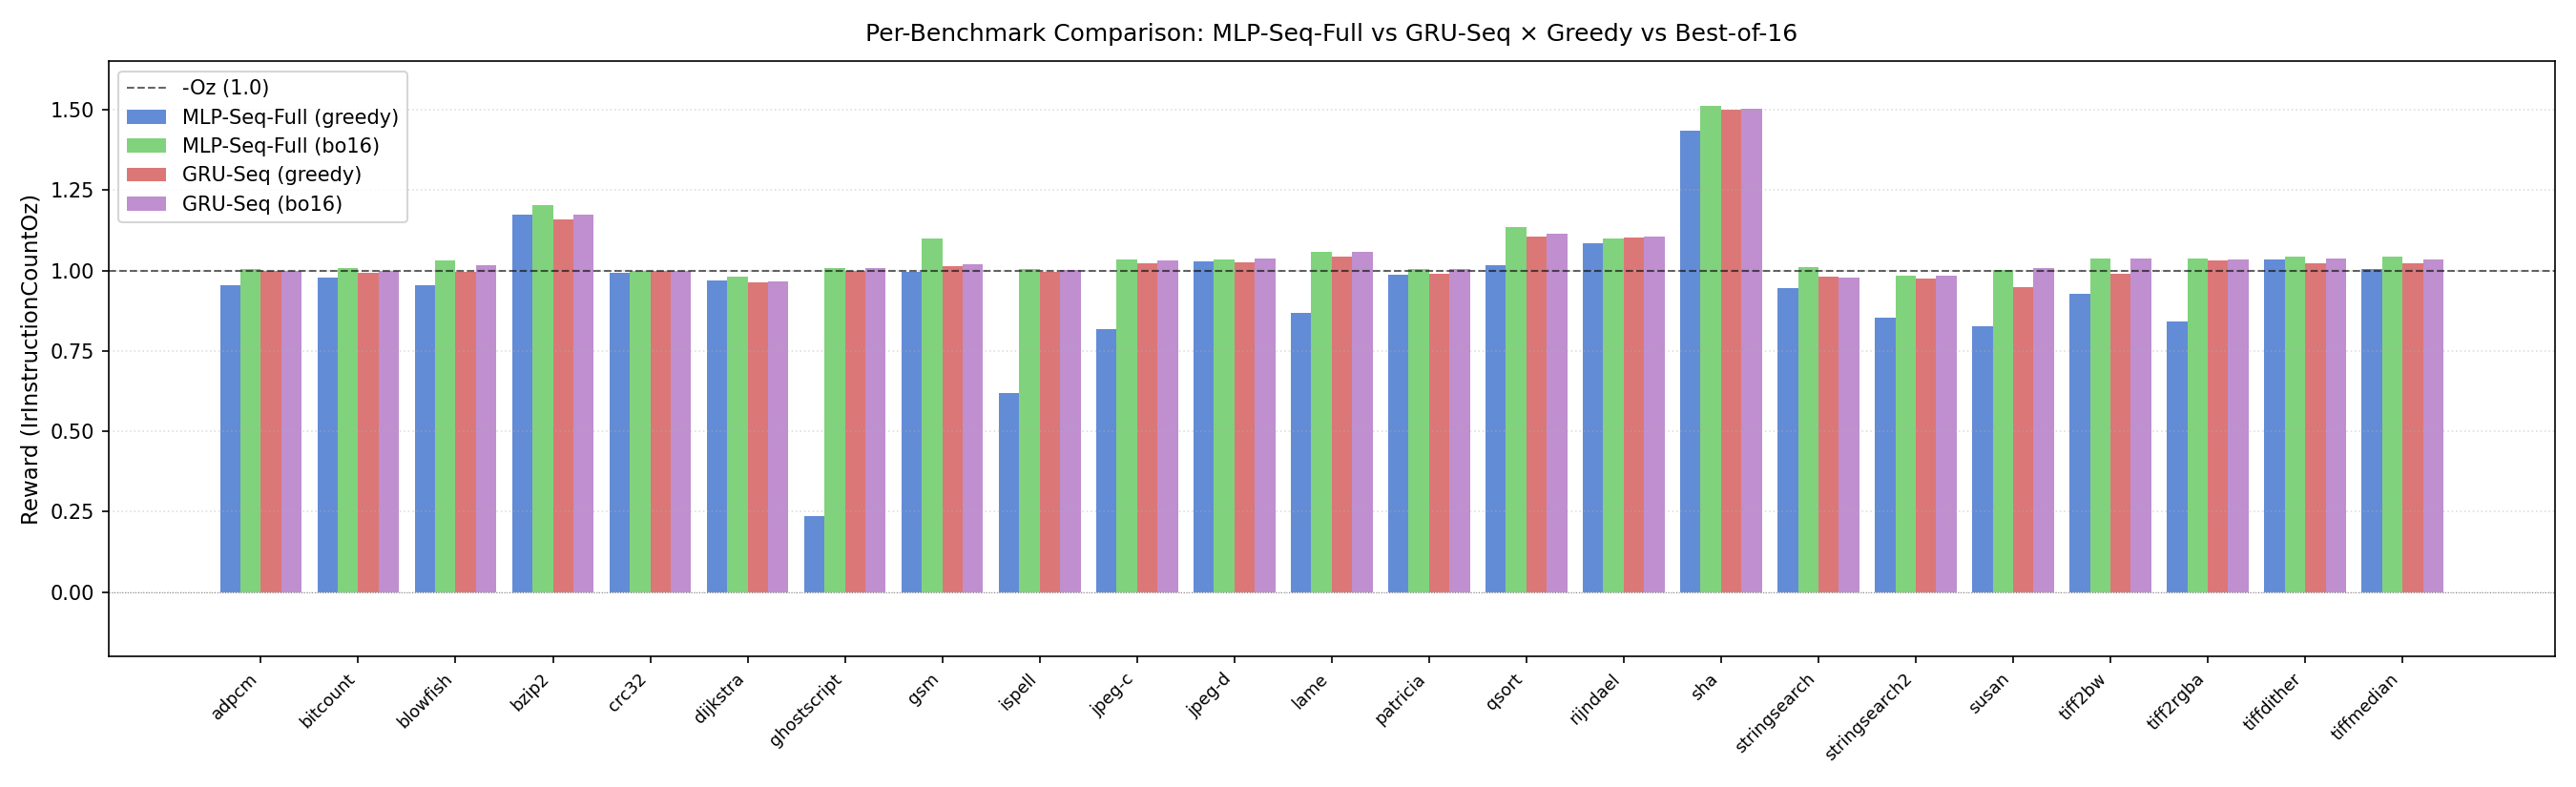
\includegraphics[width=\linewidth, height=5.5cm, keepaspectratio=false]{figures/benchmark_comparison.png}
  \caption{Per-benchmark \texttt{IrInstructionCountOz} reward for four
           configurations on all 23 \texttt{cbench-v1} benchmarks.
           The dashed line marks \texttt{-Oz} parity ($R{=}1.0$).
           Our best-of-16 (green) recovers ghostscript from greedy 0.236 to
           1.007; GRU-Seq (greedy) (red) excels on programs where the curated 30-pass
           set already contains strong optimizations.}
  \label{fig:perbench}
\end{figure}

Table~\ref{tab:main} unifies all results.
MLP-Seq-Full (bo16) (21/23) surpasses both the ensemble (ens5: 20/23) and GRU-Seq (bo16)
(18/23) on \texttt{-Oz} count, while using the same or fewer rollouts.

\textbf{Compute-budget-controlled comparison.}
MLP-Seq-Full (bo16) (16 rollouts, avg 1.060, 21/23~$\geq$Oz) substantially
outperforms random best-of-56 (56 rollouts, avg 0.992, 5/23~$\geq$Oz) and
wins on all 23 individual benchmarks, confirming that gains stem from policy
quality rather than sampling variance.\footnote{GA/SA baselines under the same
budget are natural future work.}

Notably, ghostscript---the hardest benchmark (greedy: 0.236)---reaches 1.007
under bo16, recovered by stochastic exploration over the full 124-pass space.

% ----------
\subsection{Multi-Suite Training and Reward Normalization}

\begin{figure}[h]
  \centering
  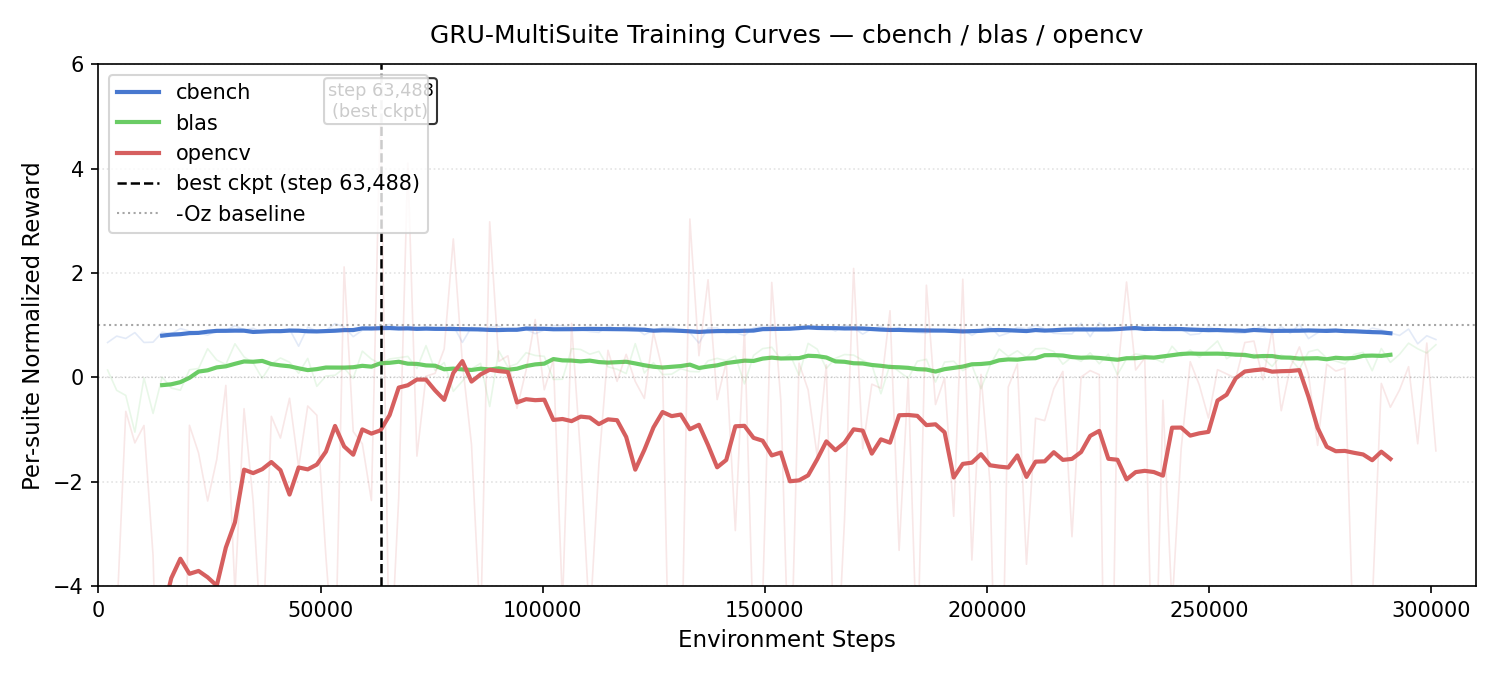
\includegraphics[width=0.92\linewidth]{figures/GRU-MultiSuite_training_curve.png}
  \caption{Per-suite normalized training return for the GRU-MultiSuite multi-suite model
           (cbench-v1: blue; blas-v0: green; opencv-v0: red).
           cbench-v1 converges earliest and most stably, crossing the
           \texttt{-Oz} parity line (dotted) around step 60k.
           opencv-v0 remains highly volatile throughout, reflecting its
           42$\times$ higher reward standard deviation relative to cbench-v1.
           The vertical dashed line marks the best global checkpoint at step
           63,488, selected before opencv-v0 noise begins degrading shared
           policy weights.}
  \label{fig:training_curve}
\end{figure}

The three suites exhibit markedly different dynamics (Figure~\ref{fig:training_curve}):
cbench-v1 peaks at $+2.45$ and converges by step 60k; blas-v0 peaks at $+3.10$
(step 85k); opencv-v0 peaks at $+1.82$ (step 110k) but remains volatile
($\sigma{=}4.44$ vs.\ cbench $\sigma{=}0.11$, a $42\times$ ratio).
The best checkpoint is selected at step 63,488 before opencv-v0 noise
destabilizes shared weights.  Without normalization, value loss diverged at
step 80k; with it, value loss stays in $[0.2, 0.8]$ throughout 300k steps.

% ----------
\subsection{Cross-Suite Generalization}

We evaluate zero-shot transfer across six additional CompilerGym benchmark
suites (full results in Appendix Table~\ref{tab:crosssuite}).
The ensemble (ens7) outperforms any single model on every suite; opencv-v0
improves from 0.20 (single model) to 2.985 (ens7), a 14$\times$
gain~\cite{lakshminarayanan2017simple}.  mibench-v1 and npb-v0 transfer
cleanly from cbench-v1 models (shared program structure).  GRU-MultiSuite multi-suite
training additionally improves blas-v0 ($0.447\to0.690$) and opencv-v0
($0.20\to1.73$) by exposing the policy to target-suite programs.
linux-v0 fails structurally: all models produce reward $-9.218$ because the
30-pass set cannot operate on kernel code with inline assembly.


% ---------------------------------------------------------------
\section{Conclusion}

We have shown that traditional DRL can learn effective compiler pass-ordering
policies that substantially outperform \texttt{-Oz} without any LLM component.
Our systematic ablation establishes that \texttt{pass\_sequence}---encoding the
ordered history of recent passes---is the dominant design choice, outperforming
IR-feature-based alternatives by a large margin.  Crucially, this finding is
\emph{architecture-independent}: adding pass\_sequence to the GRU-based policy
(GRU-Base$\to$GRU-Seq) produces the same pattern of improvement (+3.9pp greedy, +3 more
programs beating \texttt{-Oz}), independently replicating the ablation result
across two systems developed in parallel.

A cross-architecture analysis further reveals two \emph{complementary}
strengths: the curated 30-pass action set enables reliable greedy performance
(GRU-Seq: 1.038, 12/23), while stochastic inference over the full 124-pass space
recovers hard programs like ghostscript (our bo16: 1.060, 21/23).  Combining
curated passes with stochastic inference is a direct target for future work.

Scaling with parallel rollouts, truncation-aware GAE, and an inference-time
ensemble further doubles the programs beating \texttt{-Oz} versus the PPO
baseline (10$\to$20/23) and generalizes zero-shot across six OOD suites.  A
budget-controlled comparison (PPO bo16 vs.\ random bo56) confirms all gains
stem from policy quality: our policy wins on all 23 benchmarks with 3.5$\times$
fewer rollouts.

\paragraph{Limitations.}
Due to computational constraints, we do not compare against classical heuristic
search methods (GA, SA, MCTS) or beam search under the same rollout budget.
A fair comparison requires controlling for the total number of compiler
invocations; our random best-of-56 baseline establishes the sampling ceiling,
but structured search methods under the same budget remain an open comparison.
The combination of curated action set with stochastic best-of-$N$ inference is
hypothesized to be stronger than either alone but is not directly evaluated.
The 30-pass action set is incompatible with linux-v0 kernel code.  Within the
current PPO + sequence-representation design space, performance is near
saturation; future work should explore graph IR encoders
(ProGraML~\cite{cummins2021programl}) or transformer sequence models.


% ---------------------------------------------------------------
% MEMBER WORKLOAD — camera-ready only, do NOT include in submission.
%
% \section*{Member Workload}
%
% \textbf{B12508026 戴偉璿 (Wei-Hsuan Tai)} designed and conducted all
% Phase~1 ablation experiments (Sections~4.2--4.5): state representation
% (6 candidates), sequence window $k$, network architecture, PPO
% hyperparameters, and reward function comparison, running on an NVIDIA RTX
% 5070 Ti.  He identified \texttt{pass\_sequence} ($k{=}10$) as the
% strongest state representation in our evaluated design space, established
% the compute-budget-controlled comparison against random best-of-56, and
% conducted the full 23-benchmark evaluation.  He also wrote the Related
% Work, Methodology, and Experiments sections of this paper.
%
% \textbf{B12902003 馬定璿 (Ting-Xuan Ma)} [describe contribution].
%
% \textbf{B12902004 鄧育翔 (Yu-Siang Deng)} [describe contribution].
%
% \textbf{B12902033 李尚哲 (Shang-Che Li)} developed the Phase~2 training
% infrastructure and ensemble system (Sections~3.3--3.7), including
% truncation-aware GAE, 8-worker parallel rollout collection (7.6$\times$
% speedup), the 30-pass PASSES\_V4 action set, ICM exploration, per-suite
% Welford reward normalization (GRU-MultiSuite), and the seven-model
% inference-time ensemble.  He conducted cross-suite evaluation across six
% out-of-distribution benchmark suites and the multi-suite training
% experiments, running on an Apple Mac mini M4 Pro (24\,GB unified memory).
% He also wrote the Introduction.
%
% \textbf{R14944011 盧韋仲 (Wei-Chung Lu)} [describe contribution].

% ---------------------------------------------------------------
\begin{ack}
  % Omit in anonymized submission.
\end{ack}

% ---------------------------------------------------------------
\bibliographystyle{abbrvnat}
\bibliography{refs}

% ---------------------------------------------------------------
\section*{NeurIPS Paper Checklist}

\begin{enumerate}

\item {\bf Claims}
    \item[] Question: Do the main claims made in the abstract and introduction accurately reflect the paper's contributions and scope?
    \item[] Answer: \answerYes{}
    \item[] Justification: The abstract and introduction clearly state the three main contributions (state representation design, truncation-aware GAE, inference-time ensemble) and report the corresponding quantitative results (mean reward, programs beating \texttt{-Oz}). All claims are directly supported by experiments in Section~4, including a cross-architecture evaluation (Section~4.5) where the proposed \texttt{pass\_sequence} feature is integrated into a recurrent GRU baseline, demonstrating its architectural robustness and independently replicating the ablation finding across two systems developed in parallel.
    
\item {\bf Limitations}
    \item[] Question: Does the paper discuss the limitations of the work performed by the authors?
    \item[] Answer: \answerYes{}
    \item[] Justification: Section~5 (Conclusion) includes a dedicated Limitations paragraph discussing the absence of GA/SA/MCTS baselines under controlled compute budget, the structural failure of the 30-pass action set on \texttt{linux-v0} kernel code, and the saturation of the current PPO design space.

\item {\bf Theory assumptions and proofs}
    \item[] Question: For each theoretical result, does the paper provide the full set of assumptions and a complete (and correct) proof?
    \item[] Answer: \answerNA{}
    \item[] Justification: This paper presents no theoretical results; all contributions are empirical.

\item {\bf Experimental result reproducibility}
    \item[] Question: Does the paper fully disclose all the information needed to reproduce the main experimental results of the paper to the extent that it affects the main claims and/or conclusions of the paper (regardless of whether the code and data are provided or not)?
    \item[] Answer: \answerYes{}
    \item[] Justification: Section~4.1 specifies all PPO hyperparameters ($\varepsilon{=}0.2$, $\gamma{=}0.99$, $\lambda{=}0.95$, n\_steps, entropy coefficient, network architecture), the action set, reward space, episode length, and number of training episodes for both Phase~1 (MLP) and Phase~2 (GRU) architectures. The environment (CompilerGym \texttt{llvm-v0}, \texttt{cbench-v1}) is publicly available under the Apache 2.0 license.

\item {\bf Open access to data and code}
    \item[] Question: Does the paper provide open access to the data and code, with sufficient instructions to faithfully reproduce the main experimental results, as described in supplemental material?
    \item[] Answer: \answerNo{}
    \item[] Justification: Code is not released with this submission due to double-blind anonymity requirements. The benchmark data (\texttt{cbench-v1}) is publicly available through CompilerGym~\cite{CompilerGym}. All hyperparameters, network architectures, and implementation details required for reproduction are fully specified in Section~4.1 and the PPO configuration table. Code will be released upon acceptance.

\item {\bf Experimental setting/details}
    \item[] Question: Does the paper specify all the training and test details (e.g., data splits, hyperparameters, how they were chosen, type of optimizer) necessary to understand the results?
    \item[] Answer: \answerYes{}
    \item[] Justification: Section~4.1 provides full training details for both architectures: Phase~1 uses a feed-forward 256$\times$256 MLP over the full 124-pass action space (500 episodes per benchmark, NVIDIA RTX 5070 Ti), and Phase~2 uses a recurrent GRU over the curated 30-pass action space (300k steps, 8 parallel workers, Apple Mac mini M4 Pro). Hyperparameters were chosen via the systematic ablation studies in Sections~4.2--4.4, covering sequence window $k$, network capacity, n\_steps, and entropy coefficient.

\item {\bf Experiment statistical significance}
    \item[] Question: Does the paper report error bars suitably and correctly defined or other appropriate information about the statistical significance of the experiments?
    \item[] Answer: \answerNo{}
    \item[] Justification: Error bars over multiple training seeds are omitted due to the high computational cost of the compiler environment. However, to establish statistical significance, Section~4.6 introduces a compute-budget-matched baseline (Random best-of-56) that gives the random policy $3.5\times$ more rollouts than our PPO (56 vs.\ 16). Our learned policy outperforms this stronger baseline on all 23 benchmarks (avg 1.060 vs.\ 0.992), providing strong evidence that gains stem from policy knowledge rather than sampling variance. The ablation study further evaluates each configuration across all 23 \texttt{cbench-v1} benchmarks, and the count of programs beating \texttt{-Oz} provides a distribution-free summary statistic.

\item {\bf Experiments compute resources}
    \item[] Question: For each experiment, does the paper provide sufficient information on the computer resources (type of compute workers, memory, time of execution) needed to reproduce the experiments?
    \item[] Answer: \answerYes{}
    \item[] Justification: Phase~1 ablation experiments (Sections~4.2--4.4) and the compute-budget comparison (Section~4.6) were conducted on a machine with an \textbf{NVIDIA RTX 5070 Ti} GPU (500 episodes per benchmark). Phase~2 ensemble training and cross-suite evaluation (Sections~4.7--4.8) were conducted on an \textbf{Apple Mac mini M4 Pro} (24\,GB unified memory) using 8 parallel CPU workers, where each 300k-step training run completes in approximately 47 minutes. Cross-architecture validation (Section~4.5) uses the Phase~2 hardware for GRU-Base、GRU-Seq、GRU-Seq-Full.

\item {\bf Code of ethics}
    \item[] Question: Does the research conducted in the paper conform, in every respect, with the NeurIPS Code of Ethics?
    \item[] Answer: \answerYes{}
    \item[] Justification: This work studies compiler optimization, a purely technical domain with no human subjects, sensitive data, or dual-use concerns. The research conforms with the NeurIPS Code of Ethics.

\item {\bf Broader impacts}
    \item[] Question: Does the paper discuss both potential positive societal impacts and negative societal impacts of the work performed?
    \item[] Answer: \answerNA{}
    \item[] Justification: This work improves compiler optimization efficiency, which has broadly positive effects (reduced energy consumption, faster software). There are no foreseeable negative societal impacts from automated compiler pass ordering.

\item {\bf Safeguards}
    \item[] Question: Does the paper describe safeguards that have been put in place for responsible release of data or models that have a high risk for misuse (e.g., pre-trained language models, image generators, or scraped datasets)?
    \item[] Answer: \answerNA{}
    \item[] Justification: This paper poses no misuse risks. The trained models are compiler optimization policies operating solely within the LLVM compiler infrastructure, with no dual-use potential.

\item {\bf Licenses for existing assets}
    \item[] Question: Are the creators or original owners of assets (e.g., code, data, models), used in the paper, properly credited and are the license and terms of use explicitly mentioned and properly respected?
    \item[] Answer: \answerYes{}
    \item[] Justification: CompilerGym~\cite{CompilerGym} and the \texttt{cbench-v1} benchmark suite are cited in the paper and used in accordance with the Apache 2.0 license. All other third-party dependencies (PyTorch, Stable-Baselines3) are similarly open-source and used within their respective license terms.

\item {\bf New assets}
    \item[] Question: Are new assets introduced in the paper well documented and is the documentation provided alongside the assets?
    \item[] Answer: \answerNA{}
    \item[] Justification: This paper does not release new datasets or pretrained model weights. The primary contributions are algorithmic: the \texttt{pass\_sequence} state representation, the truncation-aware GAE implementation, and the inference-time ensemble strategy. Implementation details sufficient for re-implementation are provided in Sections~3 and~4.

\item {\bf Crowdsourcing and research with human subjects}
    \item[] Question: For crowdsourcing experiments and research with human subjects, does the paper include the full text of instructions given to participants and screenshots, if applicable, as well as details about compensation (if any)?
    \item[] Answer: \answerNA{}
    \item[] Justification: This paper does not involve crowdsourcing or human subjects.

\item {\bf Institutional review board (IRB) approvals or equivalent for research with human subjects}
    \item[] Question: Does the paper describe potential risks incurred by study participants, whether such risks were disclosed to the subjects, and whether Institutional Review Board (IRB) approvals (or an equivalent approval/review based on the requirements of your country or institution) were obtained?
    \item[] Answer: \answerNA{}
    \item[] Justification: This paper does not involve human subjects research.

\item {\bf Declaration of LLM usage}
    \item[] Question: Does the paper describe the usage of LLMs if it is an important, original, or non-standard component of the core methods in this research?
    \item[] Answer: \answerNA{}
    \item[] Justification: LLMs are not used in the core methodology of this work. The paper explicitly positions itself as a traditional DRL alternative to LLM-based compiler optimization approaches (Section~2.2), and all policy networks are conventional MLP and GRU architectures trained with PPO.

\end{enumerate}

% ---------------------------------------------------------------
\appendix

\section{Cross-Suite Generalization Results}

\begin{table}[h]
  \caption{Mean reward (bo8) across seven CompilerGym benchmark suites (zero-shot).
           Phase~1/2 models trained on \texttt{cbench-v1}; GRU-MultiSuite additionally on
           blas-v0 and opencv-v0.  \textbf{Bold}: best per suite.}
  \label{tab:crosssuite}
  \centering
  \begin{tabular}{lccccccc}
    \toprule
    Method & cbench & mibench & blas & npb & chstone & opencv & angha \\
    \midrule
    Random           & 0.681 & ---   & ---   & ---   & ---   & ---   & ---  \\
    PPO-Baseline           & 1.015 & ---   & ---   & ---   & ---   & ---   & ---  \\
    Best single (GRU-Seq) & 1.042 & 1.028 & 0.447 & 4.45  & 1.10  & 0.20  & 0.44 \\
    GRU-MultiSuite (bo8)        & 1.040 & 1.020 & 0.690 & 4.14  & 1.11  & 1.73  & 1.08 \\
    ens5             & 1.050 & 1.030 & 0.967 & 4.520 & 1.112 & 2.869 & 1.079 \\
    \textbf{ens7}    & 1.049 & 1.030 & \textbf{0.976} & 4.528 &
      \textbf{1.113} & \textbf{2.985} & \textbf{1.090} \\
    \bottomrule
  \end{tabular}
\end{table}

\end{document}